\section{Numerical-Domain Diagnostics}
\label{app:numerical-domain-diagnostics}

\subsection{Choice of the Primary Computational Domain}
\label{app:domain-choice}

The primary computational domain is \(A_0=[-1,3]\), evaluated on 41 equally spaced candidate values with step size \(h=0.1\). This domain is retained from the preserved Monte Carlo implementation rather than chosen after observing the results of the weak-instrument extension. Using the same domain for all sample sizes, quantiles, instrument-relevance settings, and estimators makes the accepted-set measures directly comparable across the simulation design.

The interval also contains the true structural quantile effects for all five quantiles considered in the thesis. Under the data-generating process,
\[
\alpha_0(\tau)=1+\Phi^{-1}(\tau),
\]
so the true effects are approximately \(-0.282\), \(0.326\), \(1.000\), \(1.674\), and \(2.282\) for \(\tau=0.10,0.25,0.50,0.75,\) and \(0.90\), respectively. Thus, none of the true parameter values lies close to or outside the boundaries of \(A_0\). The interval should therefore be understood as a common numerical search domain, not as an assumed theoretical parameter space.

A finite search domain can nevertheless become restrictive when instruments are weak and many candidate values are accepted. For this reason, a separate sensitivity diagnostic expands the search range from \(A_0=[-1,3]\) to \(A_1=[-3,5]\) and then to \(A_2=[-5,7]\). Under strong instrument relevance, expanding the domain adds little accepted measure, indicating that the observed accepted components are well localized within the investigated ranges. At intermediate relevance, the wider domains contain additional accepted values in some profiles. Under the weakest relevance setting, the accepted measure continues to increase as the domain is expanded and does not stabilize within \(A_2\).

These results clarify the interpretation of the main accepted-set measure. A value close to four in \(A_0\) means that almost the entire four-unit primary domain is accepted; it does not mean that the unrestricted confidence region has length four. Similarly, continued acceptance in the wider domains indicates poor numerical localization over the ranges examined, but it does not by itself establish that the theoretical confidence region is globally unbounded or that identification completely fails.

Table~\ref{tab:appendix-grid-measures} retains the key frozen domain-measure comparisons; Figure~\ref{fig:grid-domain} summarizes the expansion pattern.

\begingroup
\begin{booktabs}[
  caption = {Grid-domain diagnostic: accepted-set measures},
  label = {tab:appendix-grid-measures},
  long,
  remark{Note} = {Domains are $A_0=[-1,3]$, $A_1=[-3,5]$, and $A_2=[-5,7]$. Diagnostics concern only these investigated numerical domains and do not establish global boundedness, unboundedness, or disconnected components.}
]{
  colspec = {Q[c] Q[c] Q[c] X[l] *{6}{Q[r]}},
  columns = {colsep = 1pt},
  row{1} = {font = \bfseries},
  rowhead = 1
}
$n$ & $\tau$ & $\kappa$ & Estimator & Med. $A_0$ & Med. $A_1$ & Med. $A_2$ & Mean $A_0$ & Mean $A_1$ & Mean $A_2$ \\
1000 & 0.10 & 1.00 & Oracle-GMM & 0.400 & 0.400 & 0.400 & 0.386 & 0.386 & 0.386 \\
1000 & 0.10 & 1.00 & Full-GMM & 0.800 & 0.800 & 0.800 & 0.757 & 0.757 & 0.757 \\
1000 & 0.10 & 1.00 & DML-IVQR-BC & 0.600 & 0.600 & 0.600 & 0.705 & 0.705 & 0.705 \\
1000 & 0.10 & 0.25 & Oracle-GMM & 3.400 & 5.325 & 7.250 & 3.019 & 4.994 & 6.838 \\
1000 & 0.10 & 0.25 & Full-GMM & 3.375 & 5.950 & 8.200 & 3.304 & 5.774 & 8.037 \\
1000 & 0.10 & 0.25 & DML-IVQR-BC & 3.750 & 5.950 & 7.950 & 3.607 & 6.040 & 8.245 \\
1000 & 0.10 & 0.10 & Oracle-GMM & 4.000 & 7.900 & 11.900 & 3.745 & 7.381 & 11.002 \\
1000 & 0.10 & 0.10 & Full-GMM & 3.900 & 7.800 & 11.600 & 3.785 & 7.394 & 10.975 \\
1000 & 0.10 & 0.10 & DML-IVQR-BC & 4.000 & 7.575 & 10.775 & 3.845 & 7.219 & 10.339 \\
1000 & 0.25 & 1.00 & Oracle-GMM & 0.300 & 0.300 & 0.300 & 0.259 & 0.259 & 0.259 \\
1000 & 0.25 & 1.00 & Full-GMM & 0.400 & 0.400 & 0.400 & 0.429 & 0.429 & 0.429 \\
1000 & 0.25 & 1.00 & DML-IVQR-BC & 0.300 & 0.300 & 0.300 & 0.346 & 0.346 & 0.346 \\
1000 & 0.25 & 0.25 & Oracle-GMM & 2.175 & 2.800 & 2.850 & 2.224 & 3.158 & 3.964 \\
1000 & 0.25 & 0.25 & Full-GMM & 2.450 & 3.500 & 4.075 & 2.517 & 3.768 & 4.745 \\
1000 & 0.25 & 0.25 & DML-IVQR-BC & 2.750 & 4.650 & 6.225 & 2.630 & 4.130 & 5.712 \\
1000 & 0.25 & 0.10 & Oracle-GMM & 3.900 & 7.700 & 11.500 & 3.492 & 6.699 & 9.872 \\
1000 & 0.25 & 0.10 & Full-GMM & 3.825 & 7.600 & 11.100 & 3.595 & 6.891 & 10.083 \\
1000 & 0.25 & 0.10 & DML-IVQR-BC & 4.000 & 7.700 & 11.125 & 3.651 & 6.926 & 9.984 \\
1000 & 0.50 & 1.00 & Oracle-GMM & 0.200 & 0.200 & 0.200 & 0.235 & 0.235 & 0.235 \\
1000 & 0.50 & 1.00 & Full-GMM & 0.400 & 0.400 & 0.400 & 0.373 & 0.373 & 0.373 \\
1000 & 0.50 & 1.00 & DML-IVQR-BC & 0.300 & 0.300 & 0.300 & 0.259 & 0.259 & 0.259 \\
1000 & 0.50 & 0.25 & Oracle-GMM & 1.875 & 2.200 & 2.200 & 1.960 & 2.682 & 3.229 \\
1000 & 0.50 & 0.25 & Full-GMM & 2.250 & 2.400 & 2.550 & 2.368 & 3.171 & 3.802 \\
1000 & 0.50 & 0.25 & DML-IVQR-BC & 1.950 & 2.500 & 3.025 & 2.124 & 3.020 & 3.942 \\
1000 & 0.50 & 0.10 & Oracle-GMM & 3.825 & 7.600 & 11.300 & 3.521 & 6.640 & 9.687 \\
1000 & 0.50 & 0.10 & Full-GMM & 3.900 & 7.625 & 11.450 & 3.536 & 6.718 & 9.817 \\
1000 & 0.50 & 0.10 & DML-IVQR-BC & 3.900 & 7.500 & 10.325 & 3.538 & 6.671 & 9.585 \\
1000 & 0.75 & 1.00 & Oracle-GMM & 0.300 & 0.300 & 0.300 & 0.290 & 0.290 & 0.290 \\
1000 & 0.75 & 1.00 & Full-GMM & 0.500 & 0.500 & 0.500 & 0.512 & 0.512 & 0.512 \\
1000 & 0.75 & 1.00 & DML-IVQR-BC & 0.300 & 0.300 & 0.300 & 0.279 & 0.279 & 0.279 \\
1000 & 0.75 & 0.25 & Oracle-GMM & 2.825 & 4.200 & 4.850 & 2.628 & 3.945 & 4.990 \\
1000 & 0.75 & 0.25 & Full-GMM & 2.950 & 4.450 & 5.150 & 2.827 & 4.267 & 5.478 \\
1000 & 0.75 & 0.25 & DML-IVQR-BC & 2.325 & 3.300 & 3.900 & 2.402 & 3.595 & 4.788 \\
1000 & 0.75 & 0.10 & Oracle-GMM & 3.975 & 7.750 & 11.700 & 3.670 & 6.999 & 10.357 \\
1000 & 0.75 & 0.10 & Full-GMM & 3.900 & 7.750 & 11.500 & 3.661 & 7.023 & 10.267 \\
1000 & 0.75 & 0.10 & DML-IVQR-BC & 3.900 & 7.350 & 10.375 & 3.554 & 6.691 & 9.736 \\
1000 & 0.90 & 1.00 & Oracle-GMM & 0.500 & 0.500 & 0.500 & 0.519 & 0.519 & 0.519 \\
1000 & 0.90 & 1.00 & Full-GMM & 1.000 & 1.000 & 1.000 & 1.026 & 1.031 & 1.031 \\
1000 & 0.90 & 1.00 & DML-IVQR-BC & 0.400 & 0.400 & 0.400 & 0.454 & 0.454 & 0.454 \\
1000 & 0.90 & 0.25 & Oracle-GMM & 3.650 & 5.850 & 7.850 & 3.381 & 5.625 & 7.675 \\
1000 & 0.90 & 0.25 & Full-GMM & 3.675 & 6.150 & 8.575 & 3.555 & 6.123 & 8.432 \\
1000 & 0.90 & 0.25 & DML-IVQR-BC & 3.450 & 5.400 & 7.300 & 3.114 & 5.249 & 7.374 \\
1000 & 0.90 & 0.10 & Oracle-GMM & 4.000 & 7.900 & 11.800 & 3.712 & 7.241 & 10.771 \\
1000 & 0.90 & 0.10 & Full-GMM & 3.900 & 7.700 & 11.500 & 3.817 & 7.448 & 11.031 \\
1000 & 0.90 & 0.10 & DML-IVQR-BC & 4.000 & 7.700 & 11.600 & 3.644 & 7.042 & 10.395 \\
\end{booktabs}
\endgroup

\clearpage
\begin{figure}[tbp]
  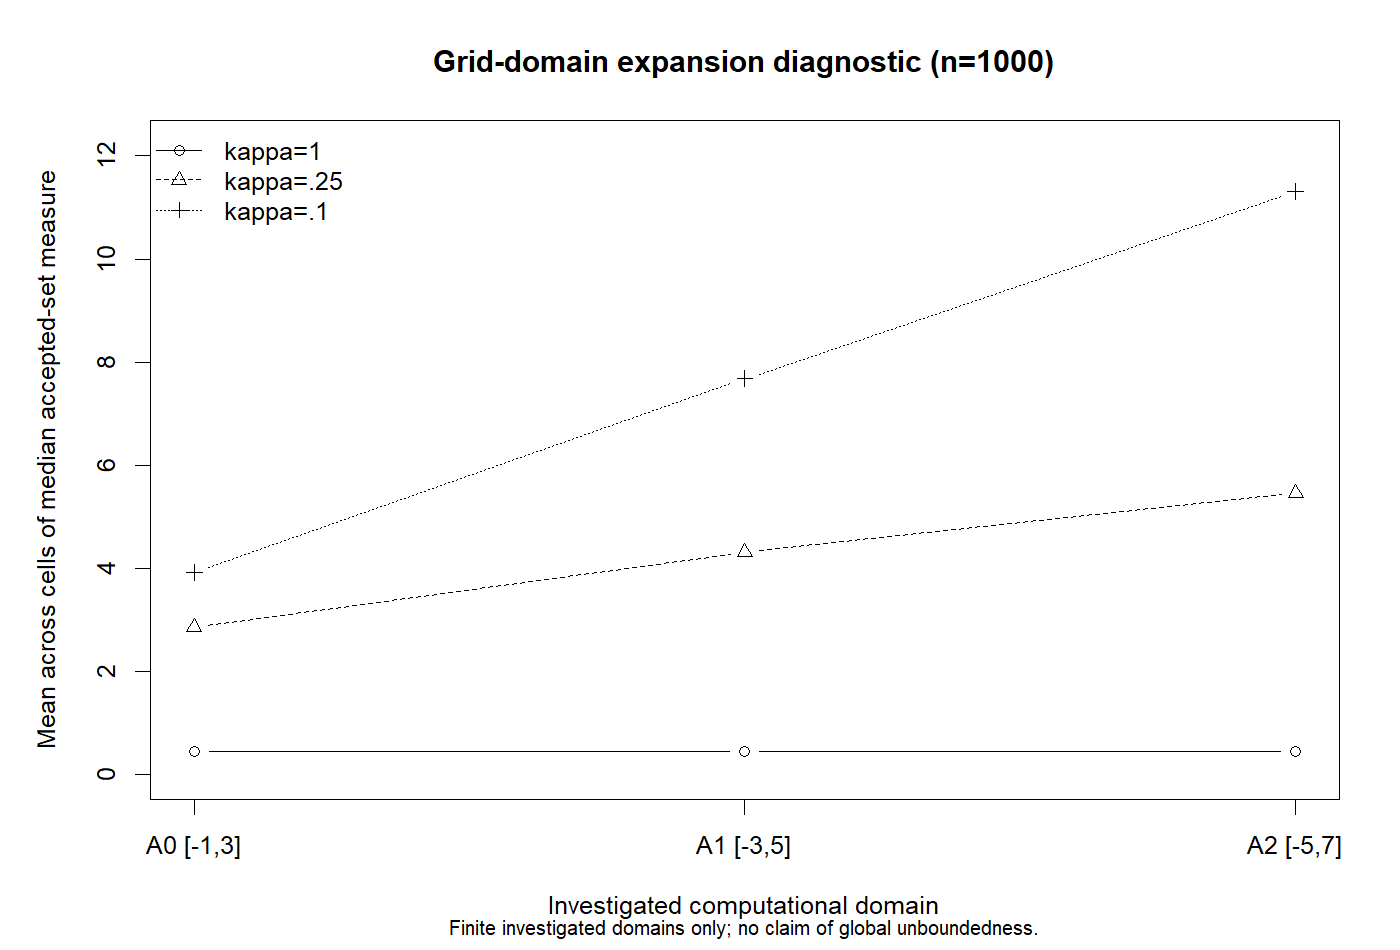
\includegraphics[width=0.88\textwidth]{figures/grid_domain_expansion.png}
  \caption{Sensitivity of the accepted set to expansion of the computational domain}
  \label{fig:grid-domain}
  \begin{figurenotes}[Note]
    The investigated domains are $A_0=[-1,3]$, $A_1=[-3,5]$, and $A_2=[-5,7]$. The diagnostic records whether the accepted set stabilizes within these numerical domains; it does not establish global boundedness or unboundedness.
  \end{figurenotes}
\end{figure}

\clearpage

\subsection{Numerical Handling of the Domain Diagnostic}

The diagnostic recorded one Stage~1 numerical failure: replication 35 at $\tau=0.90$, $\kappa=0.10$, for DML-IVQR at candidate $a=-2.1$, with a singular-design error. Stage~2 recorded no new evaluation errors. The affected profile was treated as incomplete, and its aggregate accepted-set measures were not calculated from partial information.
